\chapter{Implementation}
\label{chap:impl}


\section{Chosen programming language}
The proposed architecture of the translator implies large amounts of work with strings, and due to that, the Python programming language was chosen, as it is a language containing extensive functionality to work with text strings.
However, after the first prototype of the translator was implemented, it was found out that this language bears many difficulties in the task of implementation of the complete system. Thus it was decided to change the implementation language to Java, as it is one of the most widely used languages for multiple purposes.
After rewriting the prototype into Java, we realized that this language is all too bulky for the task --- for each new class, which were planned to be a vast multitude, it was necessary to create a separate file for the source code. 
With this issue in mind, finally the Kotlin programming language was chosen, due to it being the most suitable for the implementation: on the one hand, it is as powerful as Java, and on the other hand, as compact and expressive as Python.


\section{Prototype implementation details}
SLang is designed to be a multiparadigm programming language, so due to this fact it was decided to implement the system in a paradigm-by-paradigm fashion, starting with the simplest paradigms, then moving to more complex ones.
For a start, it was vital to implement basics of imperative programming: variable declaration and assignment, loops and branches.
After that, the next step was procedural programming --- function declaration, definition, and calls; the next one --- the introduction of OOP basics: simplistic classes, with fields and methods.
As stated in the previous chapter, there was no need to implement encapsulation, since it would unnecessarily complicate the situation, since most of the restrictions customarily forced by encapsulation are enforced over the course of analysis of the source code and AST construction. Instead, only inheritance and polymorphism were implemented. After that, it was decided to implement I/O and work with files as necessary programming elements in any language.

\section{Basic translator architecture}
All the architecture is designed in a way to implement the concept mentioned above of patterns: each pattern, which reflects one of the language constructs, is mapped to a class that implements the Constructable interface, which contains the construct() method, designed to use a pattern to substitute parameters inside it.
The language constructs, following the target language grammar, are nested, which is represented in the translator as the recursive aggregation of Constructable classes. The structure of this aggregation tree is a total copy of an input program AST.
The entry point of a program to be translated is represented with the EntryPoint class, which then contains all the other elements of the program.
The source code retrieval process launch is done via calling the construct() method, which performs a recursive walk across the aggregated instances, calling construct() inside every single one. This way, the process of the translation into the target source code is similar to AST walk, with the only difference that in this case, for every tree node the target language source code snippet is generated.

The translator source code files are split into several directories:
\begin{itemize}
    \item \textbf{language\_primitives} --- The source code files which contain basic language constructs, as well as the basic translator logic.
    \item \textbf{additional} --- Necessary utilities, used over the course of the work with translator.
    \item \textbf{mains} --- A directory for entry point files -- in each of them, there is a certain program in C, in the translator internal representation, ready for translation.
    \item \textbf{json\_patterns} --- Contains JSON-encoded patterns for different target programming languages. By now, patterns for C and JS are present.
\end{itemize}

\begin{figure}[h!]
    \centering
    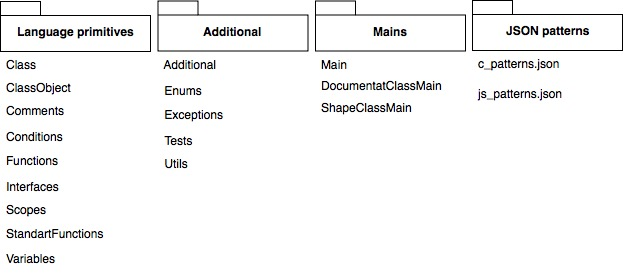
\includegraphics[width=\linewidth]{Thesis_UML.jpg}
    \caption{Project structure}
    \label{fig:Project_structure}
\end{figure}


\section{Implementation details}

\subsection{Patterns file}
The patterns file is a JSON file, which is divided into several parts:
\begin{itemize}
    \item The header part, which contains the pattern file version and a target language for the code generation. Both fields are not used for now and are rather done for the sake of future extension since the architecture allows code generation for multiple programming languages, as well as several versions of pattern files are possible.
    \item The patterns that represent the syntax of a target language.
    \item The list of standard libraries and functions contained in them: \textbf{dependencies} --- necessary for the sake of use of standard functions of a target language to project the functionality from SLang. Examples include console I/O.
    \item The list of standard functions of a target language: {standard\_functions} --- unlike the previous part, here is a place to describe every standard library function in a target language, if any. For instance, for the C programming language, we included functions printf() and scanf() as examples.
    \item A list of standard types in a target language: \textbf{standard\_types} --- to project SLang types onto the target language.
\end{itemize}

Moreover, there is a possibility of adding new sections to the format, depending on a target language and a patterns file version, depending on the evolving translator architecture. The way a pattern file looks can be seen in \ref{lst:Json_patterns}.

Such a way of pattern organization is suitable for source code generation into such languages as C, C++, Java, Kotlin, C\#, and Swift.
Moreover, over the course of translator architecture and pattern file format rework, it is theoretically possible to generate basic language constructs of languages similar to Python, JavaScript, and some others.
As an experiment, it was attempted to write patterns for JS, as well as writing a simplistic HelloWorld in it.
Results can be seen in the ``DocumentClassMain.kt'' file in ``mains'' package of the translator project directory, while a file with patterns is shown in Appendix \ref{lst:Json_JS_patterns}, as well as in the project directory.


\subsubsection{A technicality}
Since patterns are stored in a file, and disk I/O is time costly, it was decided to cache all the pattern data on the first file access, which is implemented inside the ``PatternsLoader'' class in ``Utils.kt'' in the ``additional'' package.

\subsection{Class Object}
In this implementation, in an inheritance model, for each class, virtual tables are created, along with a pointer to a parent object. Thus a natural question arises, namely what the parent of the class which is highest along the hierarchy is.
There can be two actual variants: either NULL or some class Object, which is the base class for all the created classes like it is done in Java. In SLang, the second approach was chosen, as it allows creating methods necessary for all objects, such as toString(), hashCode() and similar. Also, such approach allows not thinking about how to process the NULL parent.

\subsection{Kotlin implementation moments}
In this implementation, each language construct of a target language is mapped onto some class. 
Thanks to this architecture and Kotlin language features, the internal representation for many language constructs is implementing through inheriting from the Patternable abstract class, where the patternTyped field is overridden. The field has ``PATTERN\_TYPES'' type, which is an enum class, where each member is representative of a specific pattern.

Overall, enum classes are used quite widely in the translator. As of the time of writing, there are four of them:
\begin{itemize}
    \item \textbf{PATTERN\_TYPES} explained above, mapped ontpo patterns for every language construct;
    \item \textbf{EXPR\_TYPES}, used to denote an expression in a pattern, such as ``BODY'', ``VAR\_NAME'', ``LIB'' and similar;
    \item \textbf{STD\_TYPES} --- the list of standard types, commonly used in most of languages, such as ``INT'', ``REAL'', ``VOID'';
    \item \textbf{STD\_FUNCTIONS} --- the list of standard function concepts, existing in most of languages, such as console input and output.
\end{itemize}

\subsection{Makefile generation}
The makefile generation is done with the same technology, using patterns. The general makefile structure is shown in Appendix \ref{lst:C_make}.
Over the course of intermediate representation recompilation, the names of all source code files are put into a specially designed list, which is put into the SOURCES variable of the makefile, while the name of the file containing the entry point is put into EXECUTABLE. 
The compiler name and version is put into the CC variable, and then, necessary launch flags are optionally assigned to CFLAGS and LDFLAGS.

\section{The current implementation stats}
As of the time of writing, the following language constructs generation is implemented:
\begin{itemize}
    \item Classes, with fields, methods, and inheritance;
    \item The Object base class, as a base for all other classes;
    \item Line comments;
    \item Branching operators (if-else);
    \item Function declarations and calls;
    \item Variables: declaration, definition and usage;
    \item Imports from standard library depending on standard function calls;
    \item Standard basic I/O functionality;
\end{itemize}


\section{The structure of a resulting C project}
The structure is going as follows:
\begin{itemize}
    \item  Classes are put into source code files and headers.
    \item  Since for all classes Object is the base one, it will also be present in project files.
    \item  The makefile is generated to ensure a proper project build.
\end{itemize}


\section{The translator testing strategy}
The translator output is a sequence of strings. Thus, testing was performed as a comparison of the output to the reference strings. For each language construct, a test case was created, as a reference string for comparison. Since now there is no task of output beautification, while formatting is often changed over the course of translator implementation, it was decided to implement functionality for removal of redundant symbols from strings. This way, unit tests for the translator were implemented.